\section{Machine learning e grafi}
La relazione principale tra ML e graph analytics si trova nei dati. Questo perché nella creazione di modelli hanno un ruolo fondamentale: migliori sono i dati, meglio si comporterá il modello. 
\subsection{Data: the true challenge}
In Machine Learning sono richieste grandi quantitá di dati per ottenere buoni risultati ma le data sources sono sempre piene di errori, valori anomali e rumore. \textbf{Perché dati sbagliati sono difficili da trattare?} Perché i modelli fanno molta fatica a riconoscere se un dato non va bene per poi scartarlo, quindi puó succedere che imparino da esso imparando a sbagliare. ML é un processo di induzione: i modelli tenderanno sempre a comportarsi bene con cose che hanno effettivamente giá visto e non supporteranno cose che non esistono nei set. Se sono presenti molti errori all'interno del dataset, il modello potrebbe overfittare sul training o creare dei bias, senza essere piú in grado di generalizzare. Il modello peró imparerá sicuramente bene da un set di feature rilevanti quindi é necessario trovare un buon compromesso tra tante feature totali, poche irrilevanti. 

\subsection{Issues}
I problemi legati alla bassa qualitá dei dati determinano una serie di vincoli, sul data management per i modelli:
\begin{itemize}
    \item \textbf{Managing big data}: gestire dati provenienti da piú fonti e combinarli in un unico set, migliora molto le prestazioni in fase di apprendimento
    \item \textbf{Designing a flexible schema}: Cercare di creare uno schema del modello che fornisca la possibilità di unire più schemi eterogenei in una struttura dati unificata e omogenea che soddisfi i requisiti informativi e di navigazione. Lo schema deve evolversi facilmente in base al progetto.
    \item \textbf{Developing efficient access patterns}: velocizzare l'accesso ai dati porta ad un miglioramento del training process. Task come feature extraction, filtering, cleaning, merging e altre operazioni di preprocessing saranno piú efficienti se potranno sfruttare una potenza di accesso ai dati piú elevata.
\end{itemize}

\subsection{Performance}
Quando parliamo di \textbf{performance} nell'ambito del Machine Learning dobbiamo specificare a cosa ci stiamo riferendo:
\begin{itemize}
    \item \textbf{Predictive accuracy}
    \item \textbf{Training performance}
    \item \textbf{Prediction performance}
\end{itemize}

\subsubsection*{Predictive accuracy}
In ambito \textit{Machine Learning}, l'\textbf{accuratezza predittiva} (\textit{predictive accuracy}) è una metrica utilizzata per valutare quanto bene un modello è in grado di fare previsioni corrette su nuovi dati, ovvero su dati non visti durante la fase di addestramento.
\\
Formalmente, nel caso di un problema di classificazione, l'accuratezza è definita come la proporzione di istanze correttamente classificate sul numero totale di istanze testate. Si calcola come:
\[
\text{Accuracy} = \frac{\text{Numero di previsioni corrette}}{\text{Numero totale di previsioni}}
\]
L'accuratezza è una metrica intuitiva e utile quando le classi sono bilanciate, ma può essere fuorviante in presenza di classi sbilanciate (ad esempio, se una classe rappresenta il 95\% dei dati, un classificatore che predice sempre quella classe avrebbe il 95\% di accuratezza ma sarebbe inutile).
\\
Nei casi in cui le classi sono sbilanciate, è consigliabile usare metriche alternative o complementari, come \textit{precision}, \textit{recall}, \textit{F1-score} o l'\textit{area sotto la curva ROC} (AUC).

\subsubsection*{Training performance}
Le \textbf{prestazioni dell'addestramento} si riferiscono al tempo necessario per elaborare il modello.
\begin{itemize}  
  \item La quantità di dati da elaborare e il tipo di algoritmo utilizzato determinano sia il tempo di elaborazione che la memoria necessaria per costruire il modello predittivo.
  
  \item Chiaramente, questo problema riguarda maggiormente gli algoritmi che producono un modello come risultato della fase di addestramento. Per gli algoritmi \textit{instance-based}, i problemi di prestazioni emergono più avanti nel processo, ad esempio durante la fase di previsione.
  
  \item Nell'\textit{apprendimento batch}, il tempo di addestramento è generalmente più lungo, a causa della maggiore quantità di dati da elaborare (rispetto all'approccio di \textit{apprendimento online}, in cui l'algoritmo apprende in modo incrementale da quantità di dati più piccole).
  
  \item Anche se nell'apprendimento online la quantità di dati da processare è ridotta, la velocità con cui questi vengono elaborati influisce sulla capacità del sistema di rimanere aggiornato con gli ultimi dati disponibili, il che ha un impatto diretto sull'accuratezza delle previsioni.
\end{itemize}

\subsubsection*{Prediction performance}
Con il termine \textbf{prediction performance} intendiamo invece il tempo impiegato per fornire previsioni. 
\paragraph{Esempio} L'output del modello di machine learning potrebbe ad esempio essere un report statico una tantum per aiutare i manager a prendere decisioni strategiche o un servizio online per utenti finali. Nel primo caso, il tempo necessario per completare la fase di previsione e calcolare il modello non é un problema significativo purché il lavoro venga completato in un lasso di tempo ragionevole. Nel secondo caso, la rapiditá é importante perché influisce sulla User Experience e l'efficacia della previsione stessa. 

\newpage

\subsection{Benefit of using graphs}
L'utilitá dei grafi nel Machine Learning risiede nella possibilitá di avere dei dati organizzati meglio, un accesso piú rapido ad essi oltre ad alcuni algoritmi per implementare i parametri delle performances. 

\subsubsection*{Storing del modello}
Nell’approccio model-based al Machine Learning, il sistema apprende un modello dai dati durante la fase di training. Questo modello va salvato per essere riutilizzato senza doverlo ricostruire ogni volta. La struttura del modello dipende dall’algoritmo usato: ad esempio, nel caso dei grafi, può consistere in:
\begin{itemize}
    \item Matrici di similarità tra nodi (per modelli tipo nearest-neighbor)
    \item Mappature tra nodi e cluster (per modelli di clustering)
Questo approccio è utile per compiti come la raccomandazione o la scoperta di comunità nei grafi.
\end{itemize} 
Le dimensioni dei due modelli differiscono enormemente. Si consideri un sistema contenente 100 elementi:
\begin{itemize}
    \item Le similarità tra elementi richiederebbero l'archiviazione di 100 x 100 voci. Sfruttando le ottimizzazioni, questo numero può essere ridotto per considerare solo i primi k elementi simili quindi 100 x k voci.
    \item La mappatura tra elementi e cluster richiede solo 100 voci; pertanto, lo spazio necessario per archiviare il modello in memoria o su disco potrebbe essere enorme o relativamente modesto. Inoltre, il tempo di accesso/interrogazione del modello influisce sulle prestazioni globali durante la fase di predizione.
\end{itemize}
Per questi motivi, la gestione dell'archiviazione dei modelli rappresenta una sfida significativa nel machine learning.

\subsubsection*{Real Time}
Molti sistemi ML richiedono una risposta real time per l'utente.
\\
\begin{figure}[th]
    \centering
    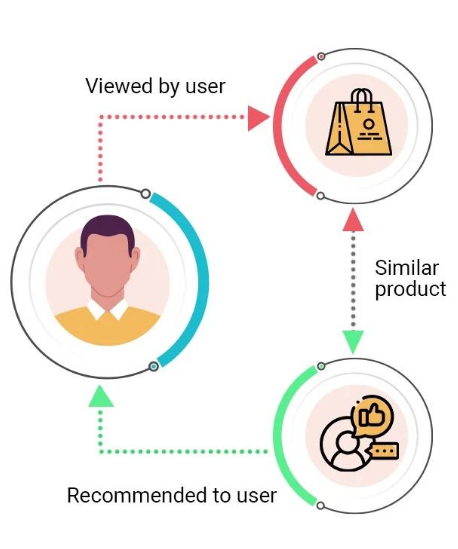
\includegraphics[width=0.20\linewidth]{ML&Graphs//img/recommendations.png}
\end{figure}
\\
\paragraph{Esempio} Semplici motori di raccomandazione che reagiscono agli ultimi clic dell’utente; auto a guida autonoma che sono state istruite a non ferire un pedone che attraversa la strada.
\\
Anche se le conseguenze in caso di errore sono molto diverse tra i due casi, in entrambi è fondamentale la capacità del sistema di apprendimento di reagire rapidamente ai nuovi stimoli provenienti dall’ambiente, per garantire la qualità del risultato finale.

\subsubsection*{Graph powered machine learning}
Di seguito vedremo quali sono quindi i benefici nell'utilizzare dei grafi per la rappresentazione dei dati elaborati dai modelli ML. Le funzionalità dei grafici sono raggruppate in tre aree principali:
\begin{itemize}
    \item \textbf{Data management:} quest'area contiene le features fornite dai grafi che aiutano i modelli ML a rapportarsi con i dati
    \item \textbf{Data analysis:} quest'area contiene feature dei grafi e algoritmi utili per learning e predicting
    \item \textbf{Data visualization:} quest'area é quella di maggiore importanza per i grafi perché possono mettere in mostra la loro utilitá e intrerpretabilitá come visual tools
\end{itemize}
\begin{figure}[th]
    \centering
    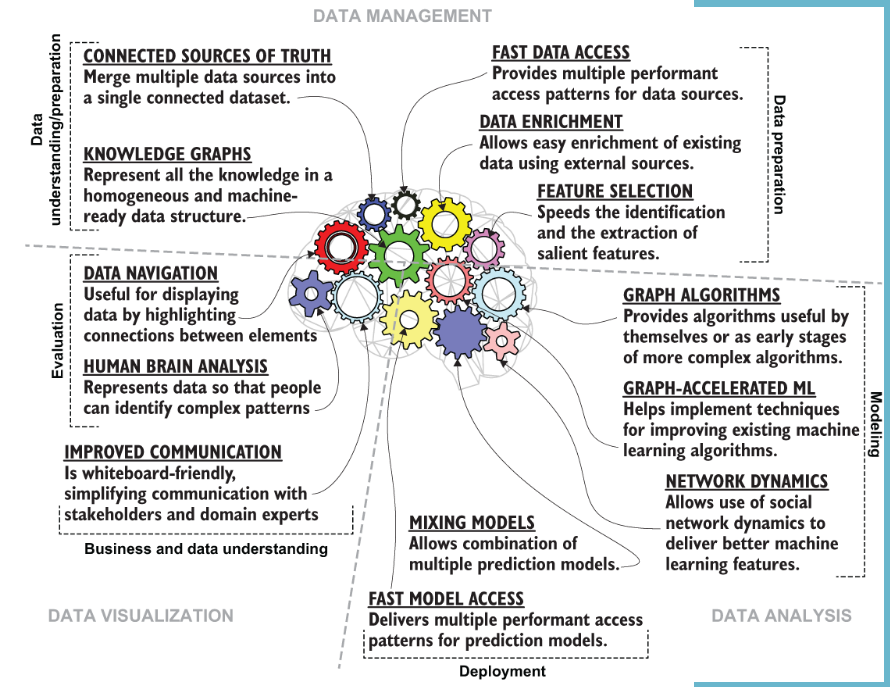
\includegraphics[width=0.65\linewidth]{ML&Graphs//img/treD.png}
\end{figure}

\paragraph{Data management} I grafi permettono ai modelli di accedere ai dati molto piú velocemente oltre a permettere una maggiore efficienza in fase di pulizia e arricchimento. Normalmente i sistemi imparano da una singola tabella, mentre i graph based possono accedere a piú di una contemporaneamente. Vediamo delle features importanti in data management fornite dai grafi: 
\begin{itemize}
    \item \textbf{Tutte le risorse sono connesse}: I grafi permetto di fare merging di multiple data sources in un singolo dataset connesso, pronto per essere usato nella fase di training. Questo riduce la data sparsity, incrementa il numero di dati disponibili e semplifica il management. 
    \item \textbf{Knowledge graph}: fornisce una data structure omogenea per combinare non solo fonti, ma anche modelli, fonti esterne... Il risultato é pronto per essere utilizzato come training, prediction o visualization. 
    \item \textbf{Accesso rapido ai dati}: differenza fondamentale tra grafo e tabella. A paritá di condizioni, un grafo rende molto piú accessibile qualunque dato, con piú relazioni che lo legano agli altri, mentre una struttura rigida a tabella é molto piú complessa.
    \item \textbf{Data enrichment}: rende semplice estendere dati pre esistenti a risorse esterne ed unirli. Questo sicuramente grazie alla natura schemaless dei grafi. 
    \item \textbf{Feature selection}: Identificare feature rilevanti é la parte fondamentale nei modelli e con un grafo hanno accesso molto rapido ad ogni tipo di dato.
\end{itemize}

\paragraph{Data analysis} I grafi possono essere utilizzati per modellare e analizzare le relazioni tra entità, così come le loro proprietà. La flessibilità dello schema offerta dai grafi permette inoltre a modelli differenti di coesistere nello stesso dataset. Le funzionalità di analisi dei dati basate su grafi includono:

\begin{itemize}
    \item \textbf{Algoritmi su grafi} — Diversi tipi di algoritmi, come il clustering, il page rank e l’analisi dei collegamenti, 
    sono utili per ottenere informazioni dai dati e per l’analisi. Inoltre, possono essere utilizzati come fase di 
    pre-elaborazione dei dati in processi di analisi più complessi.
    \item \textbf{Machine learning potenziato dai grafi}: l’estrazione di caratteristiche (feature extraction) basata su grafi è un esempio di come i grafi possano accelerare o migliorare la qualità di un sistema di apprendimento. I grafi aiutano a filtrare, pulire, arricchire e integrare i dati, sia prima che durante la fase di addestramento.
    \item \textbf{Dinamiche della rete}: essere consapevoli dei contesti circostanti e delle forze che agiscono sulle reti 
    permette non solo di comprendere le dinamiche della rete, ma anche di sfruttarle per migliorare la qualità delle previsioni. \textbf{Esempio}: in un social network, la diffusione di contenuti dipende anche da eventi esterni (es. una notizia virale). Capire queste dinamiche può aiutare a prevedere i trend.
    \item \textbf{Modelli misti}: possono coesistere più modelli nello stesso grafo, sfruttando la flessibilità e l’accesso veloce ai dati, a condizione che possano essere fusi nella fase di previsione. Questa caratteristica migliora la precisione finale. Inoltre, uno stesso modello a volte può essere riutilizzato in modi diversi. Diversi modelli (es. un modello per raccomandazioni, uno per rilevare anomalie) possono essere combinati in un unico grafo. Questo è utile quando ogni modello vede un “aspetto” diverso dello stesso dato.
    \item \textbf{Accesso veloce al modello}: l’uso in tempo reale richiede previsioni rapide, il che implica un modello 
    accessibile nel minor tempo possibile. I grafi offrono schemi di accesso adatti a questi scopi. I grafi permettono accesso efficiente a strutture complesse (es. neighborhood di un nodo, percorsi più brevi, comunità), rendendo le predizioni rapide e adattabili in tempo reale.
\end{itemize}

\paragraph{Data visualization}I grafi hanno un elevato potere comunicativo e possono mostrare più tipi di informazione contemporaneamente in un modo che il cervello umano comprende con facilità. Le funzionalità di visualizzazione dei dati basata su grafi includono:

\begin{itemize}
    \item \textbf{Navigazione dei dati}: i grafi sono molto utili per rappresentare i dati evidenziando le connessioni tra gli elementi. Possono essere usati sia come strumenti di navigazione visiva, che aiutano a esplorare i dati, sia come strumenti investigativi.
    
    \item \textbf{Analisi umano-macchina}: visualizzare i dati sotto forma di grafo permette di combinare le capacità del machine learning 
    con l’intuito umano, facilitando l’elaborazione avanzata e il riconoscimento di pattern complessi.
    
    \item \textbf{Comunicazione efficace}: i grafi, in particolare i property graph, sono “whiteboard friendly”, cioè facili da rappresentare 
    visivamente nello stesso modo in cui sono strutturati nel database. Questo riduce il divario tra la parte tecnica e la comunicazione verso esperti del dominio o stakeholder.
\end{itemize}
\textbf{Nota:} La visualizzazione dei grafi è particolarmente utile nei casi in cui le relazioni tra i dati contano più dei dati stessi, come nelle reti sociali, nell’analisi di frodi, o nei knowledge graph. [fonte GPT]

\subsection{Ruolo dei grafi nel Machine Learning}
Il ruolo dei grafi non comprende sempre tutti questi passaggi. Dipende dal motivo per cui vengono scelti, questa é una lista delle principali applicazioni. Riassumendo, potremmo vedere dei grafi in tutte e quattro le fasi del ML workflow:
\\
\begin{figure}[th]
    \centering
    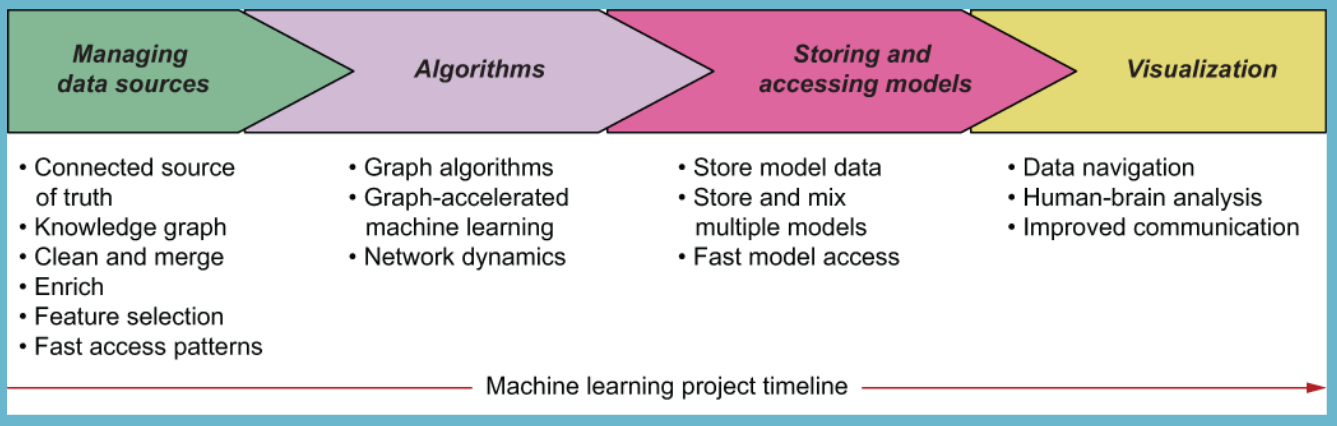
\includegraphics[width=0.75\linewidth]{ML&Graphs//img/worflow.png}
\end{figure}

\subsubsection*{ML pipeline: Managing data sources}
La trasformazione dei dati in grafi puó avvenire in diversi modi e possiamo definire due macro categorie:
\begin{itemize}
    \item \textbf{Graph modeling:} Dati convertiti in una rappresentazione a grafo. Manteniamo le stesse informazioni.
    \item \textbf{Graph construction:} Costruiamo un nuovo grafo, aggiungendo informazioni ai dati.
\end{itemize}
\subsubsection*{ML pipeline: Graph storage and learning process (Algorithms)}
\begin{figure}[th]
    \centering
    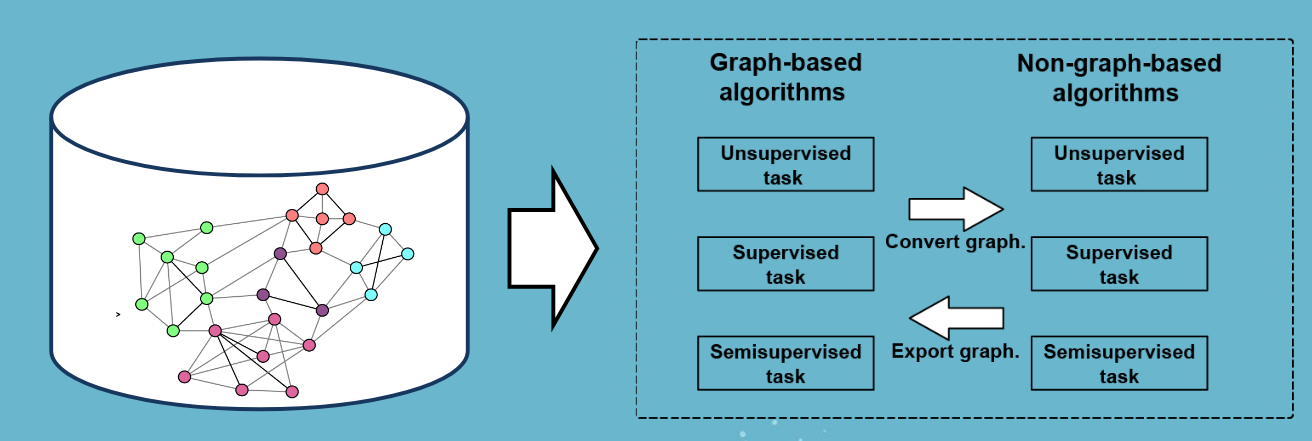
\includegraphics[width=0.6\linewidth]{ML&Graphs//img/graphstorage.png}
\end{figure}
La rappresentazione a grafo é utile per le seguenti tasks:
\begin{itemize}
  \item \textbf{Selezione delle caratteristiche}: Un grafo è facile da interrogare e può unire dati provenienti da più fonti, semplificando l'individuazione e l'estrazione delle variabili da utilizzare per l'addestramento.
  
  \item \textbf{Filtraggio dei dati}: Le relazioni facilmente navigabili tra oggetti permettono di filtrare rapidamente i dati inutili prima della fase di addestramento, velocizzando così la costruzione del modello.
  
  \item \textbf{Preparazione dei dati}: I grafi facilitano la pulizia dei dati, la rimozione di voci spurie e l'unione di dati provenienti da fonti diverse.
  
  \item \textbf{Arricchimento dei dati}: L'estensione dei dati con fonti esterne di conoscenza (come reti semantiche, ontologie e tassonomie) o l'integrazione dei risultati della fase di modellazione per costruire una base di conoscenza più ampia è semplice con un grafo.
  
  \item \textbf{Formattazione dei dati}: È possibile esportare i dati nel formato necessario: vettori, documenti, ecc.
\end{itemize}

Per selezionare l'algoritmo, decidiamo tra due approcci principali uno dove usiamo il grafo come algoritmo di learning e uno dove usiamo il grafo per semplificare una pipeline altrimenti molto piú complessa. 

\paragraph{Fast computation of similarity using graphs} Normalmente, dati due items, dovrei calcolare la cosine similarity con ogni altro elemento del dataset per capire gli elementi simili. É possibile invece implementare un metodo che sfrutti la potenza dei grafi: usare un \textbf{bigrafo (o bigraph)}. É una specie particolare di grafo i cui nodi possono essere divisi in due set U e V disgiunti e indipendenti; ogni nodo del set U si collegherá solo a nodi del set V. 
\\
\begin{figure}[th]
    \centering
    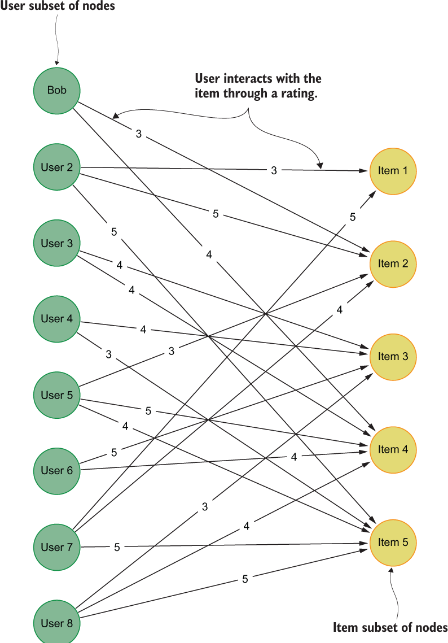
\includegraphics[width=0.4\linewidth]{ML&Graphs//img/bigraph.png}
\end{figure}
\\
\textbf{Perché conviene?} Utilizzando la rappresentazione a grafo, è facile utilizzare una semplice query per trovare tutti gli oggetti che hanno almeno un utente valutatore in comune. La similarità può quindi essere calcolata solo tra l'oggetto corrente e quelli sovrapposti, riducendo notevolmente il numero di calcoli necessari.

\subsubsection*{ML pipeline: Storing and Accessing models}
Il terzo step nel workflow consiste nel dare delle predizioni all'utente finale. Il modello deve essere salvato in modo da poter essere riutilizzato ogni volta che é richiesta una nuova prediction. La velocitá con cui accediamo al modello limita la prediction performance: il tempo é un elemento di valutazione fondamentale per un modello di ML. 
\\
Nel bigrafo ad esempio é molto semplice salvare anche la matrice di similaritá: basta infatti collegare tra loro i nodi con degli archi con il loro valore di similarity e per ridurre la complessitá tenere solo i top k.

\paragraph{Rete bayesiana} Una rete bayesiana é un grafo diretto dove ogni nodo é una variabile associata a delle informazioni probabilistiche. Questo tipo di grafo combina informazioni logiche con probabilistiche. Secondo le definizioni di Russel e Norvig:
\begin{itemize}
    \item Ogni nodo corrisponde a una variabile casuale. Queste variabili possono essere grandezze osservabili, variabili latenti, parametri incogniti o ipotesi.
    \item Gli archi rappresentano dipendenze condizionali. Se esiste un arco dal nodo X al nodo Y, X si dice genitore di Y. Il grafo non ha cicli orientati (e quindi è un grafo aciclico orientato). I nodi non connessi rappresentano variabili condizionatamente indipendenti.
    \item Ogni nodo Xi ha una distribuzione di probabilità condizionata P($x_i$, Genitori($x_i$)) che quantifica l'effetto dei genitori sul nodo. In altre parole, ogni nodo è associato a una funzione di probabilità che accetta (come input) un particolare insieme di valori per le variabili genitori del nodo e fornisce (come output) la probabilità, o la distribuzione di probabilità, se applicabile, della variabile rappresentata dal nodo.
\end{itemize}

\paragraph{Rete bayesiana dinamica} Anche chiamata \textbf{Dynamic Bayesian Network}, è una rete bayesiana che modella l'evoluzione di variabili nel tempo. Significa che una DBN collega le variabili tra un tempo $t$ e il tempo $t+1$. \\
Ad esempio supponi una variabile Posizione di un robot: una DBN può rappresentare come la Posizione al tempo $t+1$ dipende dalla Posizione al tempo $t$ e dall’Azione al tempo $t$. La versione piú semplice per una DBN é una \textbf{Markov Chain}, ovvero una struttura a grafo dove ogni nodo attuale é causa del successivo e basta, senza avere una correlazione diretta con il passato. 

\subsubsection*{ML pipeline: Visualization}
La visualizzazione viene presentata alla fine del processo, poiché visualizzare i dati dopo l'elaborazione iniziale
è molto meglio che visualizzare i dati grezzi, ma la visualizzazione dei dati può avvenire in qualsiasi momento
del workflow. L'importanza della visualizzazione dei dati risiede nell'analizzare dati complessi, identificare modelli ed estrarre informazioni preziose. Semplificare informazioni complesse e presentarle visivamente consente ai modelli di prendere decisioni informate ed efficaci in modo rapido e accurato. Inoltre la visualizzazione dei dati gioca un ruolo chiave perché ci consente di accedere e analizzare i dati da una prospettiva diversa. 
\paragraph{L'importanza della visualizzazione} Gli esseri umani sono creature naturalmente visive. I nostri occhi sono i nostri recettori sensoriali più potenti e presentare i dati attraverso la visualizzazione delle informazioni sfrutta al meglio le nostre capacità percettive. Molti set di dati oggi sono troppo grandi per essere analizzati senza strumenti computazionali che ne facilitino l'elaborazione e l'interazione. Se esploriamo i dati sotto forma di grafico, è più facile individuare pattern, valori anomali e lacune. Il modello grafico espone relazioni che potrebbero essere nascoste in altre visualizzazioni degli stessi dati (come tabelle e documenti) e ci aiuta a individuare i dettagli importanti. 
\\
\begin{figure}[th]
    \centering
    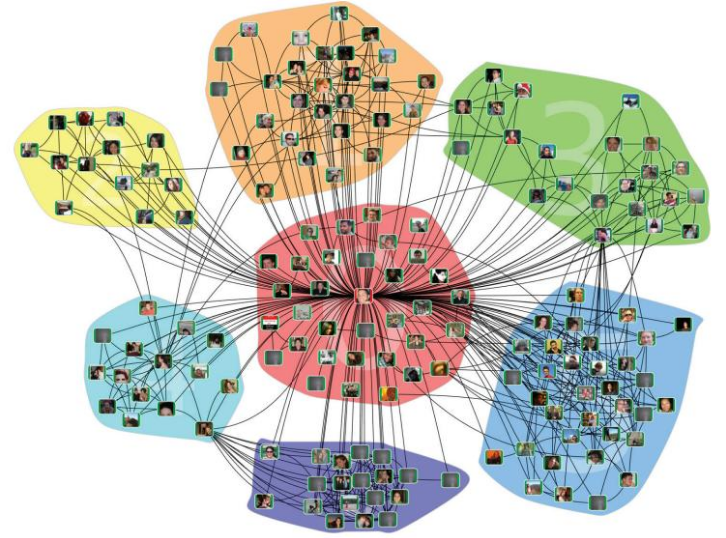
\includegraphics[width=0.5\linewidth]{ML&Graphs//img/esempiovisualiz.png}
\end{figure}
\\
Scegliere la rappresentazione migliore per un grafo non é semplice, proprio perché dev'essere ben descrittiva e non in confusione. Qui sopra si puó vedere la rappresentazione della rete di amicizie di un utente Facebook.
